\documentclass[twocolumn,Spanish,a4paper,11pt]{article}
\usepackage[spanish,es-tabla]{babel}
\usepackage[utf8]{inputenc}
\usepackage{graphicx}
\usepackage{float}
\usepackage{amsmath}
\usepackage{upgreek}
\usepackage[none]{hyphenat}
\usepackage[left=1cm,top=2.5cm,right=1cm,bottom=2.5cm]{geometry} 
\usepackage{subfig}
\usepackage[]{mcode}

\begin{document}

\twocolumn[
\centering
  \begin{@twocolumnfalse}
\begin{LARGE}
\textbf{Práctica computacional: modelo de Ising} \\
\end{LARGE}
\vspace{10pt}
%\begin{Large}

Andrés Rabinovich\\
Axel Andrés Hofele\\
Mariana Paula Scilingo\\
\today
%\end{Large}
%\hspace{15pt}

\begin{abstract}
En el presente trabajo analizamos la magnetización y la energía de una red cuadrada de espines en función
de la temperatura, empleando una simulación númerica del modelo de Ising (Montecarlo). Para ello se utilizó el
algoritmo de Metrópolis, y se consideraron condiciones de contorno periódicas. Se estudió la transición de fase del
sistema, comportándose como ferromagnético (paramagnético) para temperaturas menores (mayores) a $T_c$ $\approx$ 2,26.

\end{abstract}
\vspace{20pt}
\end{@twocolumnfalse}
]

\section{Introducción}

El modelo de Ising fue propuesto para el estudio
de la magnetización de los materiales ferromagnéticos.
Se modela al material como una cadena spines, que
pueden tomar dos valores distintos: $s_i= \pm$1. Se tiene
en cuenta también la interacción a primeros vecinos. El
hamiltoniano es:

\begin{equation}
H=-\sum_{<ij>}{Js_is_j}-\mu B\sum_{i}{s_i},
\label{hamiltoniano}
\end{equation}

donde $J$ modela la interacción y B es un campo
magnético externo. En este trabajo utilizaremos J
isótropo y constante. Se dice que cuando $J$ $>$ 0 el
material es ferromagnético y si $J$ $<$ 0 el material es
antiferromagnético.

\section{Programa de simulación del modelo de Ising}

Se escribió un código de simulación Monte Carlo del
modelo de Ising, empleando el algoritmo Metrópolis
en una red bidimensional cuadrada de espines, para
obtener una colección representativa de distintos estados
del ensamble canónico. Se impusieron condiciones de
contorno periódicas para estudiar la magnetización en el seno de un material
magnético.
El algoritmo Metrópolis se puede desglosar en:

\begin{enumerate}
\item{Se elige una configuración inicial de la red
asignando 1 o -1 a cada spin de la misma de forma
aleatoria.}
\item{Se elige una temperatura $T$.}
\item{Se elige un spin de la red y se lo invierte (la elección
puede ser aleatoria o secuencial).}
\item{Se calcula la energía de la nueva configuración y se
la compara con la energía de la configuración en el
paso anterior.}
\item{Si la energía disminuyó, se acepta la nueva
configuración del sistema.}
\item{ Si la misma no disminuyó, se acepta el nuevo estado
con probabilidad $\exp({-\beta \Delta E}$})
\item{Se itera desde el punto (3) N veces.}
\end{enumerate}

En particular nos interesa calcular cuatro variables,
la energía $U$ y la magnetización $M$, con sus respectivas
desviaciones estándar $\sigma_U$ y $\sigma_M$ estudiando su variación
en función de la temperatura $T$.
La energía se podría calcular como:

\begin{equation}
U=\sum_{n}{E_n\ p_n},
\label{energia}
\end{equation}

donde $p_n$ es la probabilidad. Mientras que $M$ es:

\begin{equation}
M=\sum_{n}{M_n\ p_n}.
\label{magnetizacion}
\end{equation}

Como cada valor de spín puede tomar únicamente
dos valores, hay un total de 2$N$ estados para una red
de $N$ espines, con lo cual calcular en forma exacta las
ecuaciones (\ref{energia}) y (\ref{magnetizacion}) puede volverse computacionalmente
costoso. Por ello, tomaremos en cuenta sólo los estados
que contribuyan mayoritariamente.

Teniendo eso en cuenta, la energía U se puede calcular
con la siguiente aproximación:

\begin{equation}
U=\frac{1}{N}\sum_{i=1}^{N}{E_i},
\label{emedia}
\end{equation}

donde $E_i$ es la energía obtenida en el i-ésimo paso.
Análogamente para $M$:

\begin{equation}
M=\frac{1}{N}\sum_{i=1}^{N}{M_i},
\label{mmedia}
\end{equation}

Además, puede demostrarse, que la susceptibilidad
magnética, definida como $\chi =\frac{\partial{M}}{\partial{B}}$  se puede calcular:

\begin{equation}
\chi=\dfrac{\beta}{N} \left( \langle M^2 \rangle - \langle M \rangle ^2 \right)
\label{ec:susc}
\end{equation}

y en forma análoga, el calor específico a volumen
constante $C_V$ =$\frac{\partial{U}}{\partial{T}}$ se puede calcular como:

\begin{equation}
C_V = \dfrac{\beta ^2}{N} \left( \langle E^2 \rangle -\langle E \rangle ^2 \right)
\label{ec:calor}
\end{equation}

Para sistemas infinitamente grandes, uno espera obtener una transición de fase para
una temperatura crítica $T_c$. Es decir, que para
temperaturas por debajo de la crítica, se observe una
fase ferromagnética, y por encima de dicha temperatura,
una fase paramagnética. Esto implica observar un
fenómeno de magnetización espontánea para el caso
ferromagnético, y una magnetización nula para el caso
paramagnético. Dicha temperatura puede estimarse
como:

\begin{equation}
T_c=\frac{2J}{k}\frac{1}{\ln\left(1+\sqrt{2}\right)}
\label{ec:tc1}
\end{equation}

donde k es la constante de Boltzmann, que al igual que
J fue definida con valor 1 en nuestro programa. Teniendo
esto en cuenta esperamos, que para redes lo suficientemente grandes, tengamos un valor $T_c$ :

\begin{equation}
T_c\approx\frac{2}{\ln\left(1+\sqrt{2}\right)}=2,269
\label{ec:tc}
\end{equation}

que es buena aproximación a medida que $N\rightarrow \infty$.

\section{Resultados}

Las primeras muestras tomadas no son representativas
del sistema físico ya que cada muestra difiere en solo
un espín. Se debe dejar al sistema llegar al equilibrio,
tomando un número de pasos suficientemente grande
(idealmente infinito). 

\subsection{Termalización}

Al comenzar el algoritmo, el sistema se encuentra en punto del espacio de fases que no tiene porque ser un estado típico del sistema en equilibrio a una cierta temperatura. Después de hacer cierto número de flipeos (invertir un spin de la red), el sistema llega a encontrarse 
en un punto del espacio de fases en el cual los valores de la energía del sistema rondan el valor más probable.

En la figura \ref{termalizacion} se muestra la termalización para una red de 64x64 spines. Se grafica la energía en función del número de flipeos a tres temperaturas distintas, T=0.1, T=2.3, T=4.5. Se observa que para T=0.1, a partir de aproximadamente 120000 flips, la energía del sistema prácticamente no varía, por lo que decidimos termalizar todas las redes con 120000 flips. Debido a que los pasos de la temperatura en el algoritmo eran pequeños, fue suficiente termalizar al comienzo del mismo una única vez para cada red.

\begin{minipage}{0.45\textwidth}									
\centering
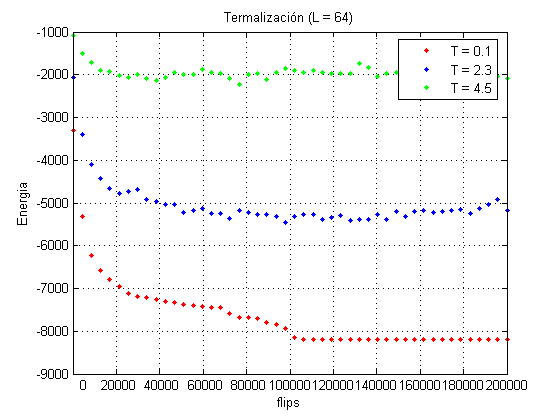
\includegraphics[totalheight=0.25\textheight]{figuras/termalizacion.png}
\captionof{figure}{Termalización en una red de L = 64}
\label{termalizacion}
\end{minipage}

\subsection{Energía media y calor específico}

En la figura \ref{grafico_energia} se graficó la energía media en función
de la temperatura para redes de 10x10,
20x20, 50x50 y 64x64. A partir
de una determinada temperatura, alrededor de 2.5, si baja la temperatura, baja la energía del
sistema. Esto sucede cuando los espines se alinean al presentarse una magnetización espontánea.

\begin{minipage}{0.45\textwidth}									
\centering
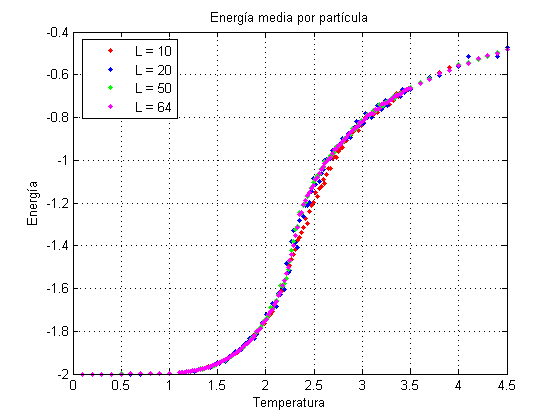
\includegraphics[totalheight=0.25\textheight]{figuras/energia.png}
\captionof{figure}{Energía media por partícula en función de la temperatura para redes de distinto lado L}
\label{grafico_energia}
\end{minipage}

Alrededor de la $T_c$ se observa un brusco cambio de
la energía del sistema junto con un cambio de concavidad en la curva de energía. Aumentando la temperatura respecto de la $T_c$, se obtiene un aumento monótono de
la energía. Asociado a este cambio brusco en la energía
alrededor de la $T_c$, debe existir un pico en el calor
específico del sistema. En la figura \ref{grafico_capacidad_calorifica} se graficó el calor
específico en función de la temperatura. Se observa un máximo alrededor de la temperatura $T_c$ para todas las redes.

\begin{minipage}{0.45\textwidth}									
\centering
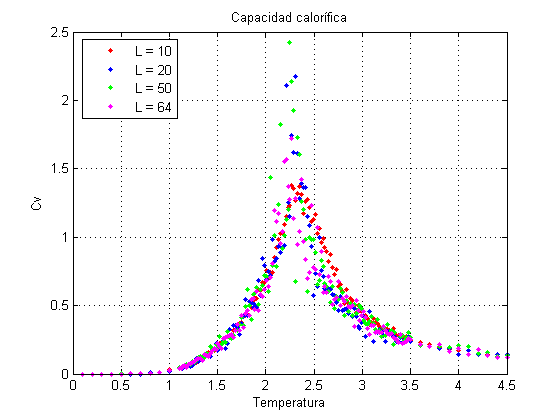
\includegraphics[totalheight=0.25\textheight]{figuras/capacidad_calorifica.png}
\captionof{figure}{Capacidad calorífica por partícula en función de la temperatura para redes de distinto lado L}
\label{grafico_capacidad_calorifica}
\end{minipage}

Para encontrar la temperatura $T_c$, se ajustó por medio de un polinomio de grado 20 el calor específico para la red de L = 64. Luego se maximizó el mismo obteniéndose un máximo en $T_c\approx2.26$, en concordancia con el calculado en \ref{ec:tc}, lo que muestra que para una red 64x64 nos encontramos prácticamente en el límite termodinámico. 
En la figura \ref{capacidad_calorifica_con_ajuste_polinomial} se observa un gráfico del calor específico para la red de L = 64 y el polinomio de ajuste. La recta vertical marca la posición del máximo encontrado.

\begin{minipage}{0.45\textwidth}									
\centering
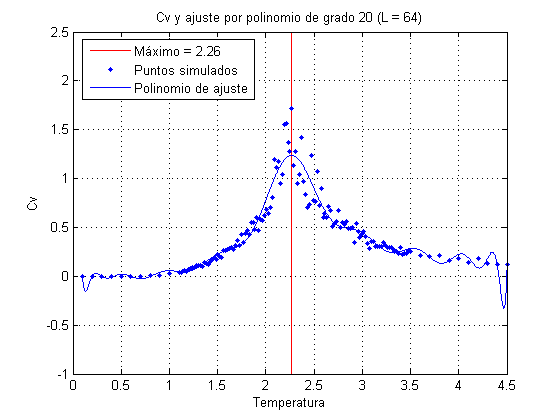
\includegraphics[totalheight=0.25\textheight]{figuras/capacidad_calorifica_con_ajuste_polinomial.png}
\captionof{figure}{Capacidad calorífica por partícula en función de la temperatura para una red de L = 64 y ajuste polinomial}
\label{capacidad_calorifica_con_ajuste_polinomial}
\end{minipage}

\subsection{Magnetización y susceptibilidad}

En la figura \ref{grafico_magnetizacion} se graficó el valor absoluto de la
magnetización media en función de la temperatura
para las cuatro redes usadas. La magnetización neta
es máxima y constante para temperaturas bajas ($T<T_c$), correspondiente a un estado del sistema con todos
los espines alineados al producirse la magnetización
espontánea, y luego se ve una súbita disminución de la magnetización
para temperaturas alrededor de la temperatura crítica
$T_c$, para luego ser prácticamente nula para temperaturas
mayores.

\begin{minipage}{0.45\textwidth}									
\centering
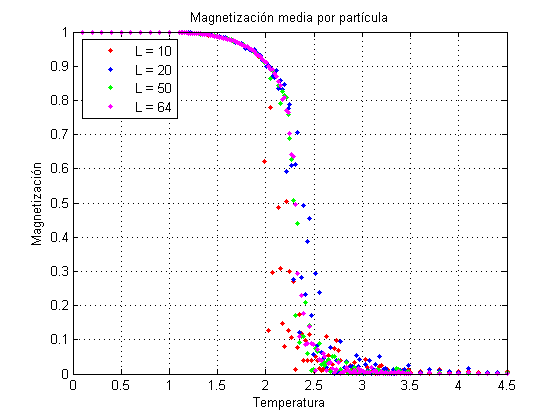
\includegraphics[totalheight=0.25\textheight]{figuras/magnetizacion.png}
\captionof{figure}{Magnetización media por partícula en función de la temperatura para redes de distinto lado L}
\label{grafico_magnetizacion}
\end{minipage}

Análogamente al caso anterior, el cambio repentino de
la magnetización se relaciona con una variación brusca en la susceptibilidad magnética. En la
figura \ref{grafico_susceptibilidad_magnetica} se graficó la susceptibilidad en función de la
temperatura, donde se observa un pico en los valores
en donde ocurre el cambio en la magnetización, en
los valores esperados para la $T_c$.

\begin{minipage}{0.45\textwidth}									
\centering
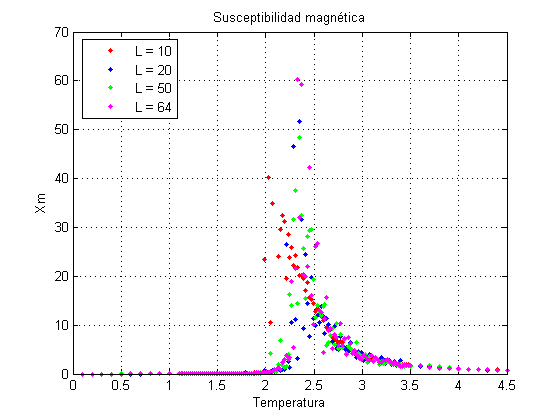
\includegraphics[totalheight=0.25\textheight]{figuras/susceptibilidad_magnetica.png}
\captionof{figure}{Susceptibilidad magnética por partícula en función de la temperatura para redes de distinto lado L}
\label{grafico_susceptibilidad_magnetica}
\end{minipage}

\subsection{Efectos de tamaño finito y temperatura
crítica}

Los efectos de tamaño finito se deben a que las
muestras usadas en la simulación tiene un número
de espines pequeño en comparación con el límite
termodinámico.

Para los sistemas de 10x10 y 20x20 espines,
observamos que el valor medio de la magnetización
por espín varía suavemente desde valores cercanos a
cero, para temperaturas mayores que $T_c$, a valores
prácticamente iguales a 1 para temperaturas cercanas
a cero. Es decir, no existe un cambio abrupto en el
valor de la magnetización para $T_c$, que es lo que se
espera observar en sistemas con número de espines muy
grande. Al aumentar el número de espines, notamos
que el sistema tiene un comportamiento que tiende
al esperado en límite termodinámico. En los gráficos
de magnetización media por espín para sistemas de
50x50 y 64x64, observamos que la curva tiene un
cambio cada más abrupto y menos suave, a partir de
$T\approx 2.26$. Para el valor de la
energía media no se observan diferencias significativas
al cambiar el tamaño del sistema.

\section{Conclusiones}

Se estudió el comportamiento de la magnetización,
la energía media, el calor específico y la susceptibilidad
magnética de una red cuadrada de espines en función
la temperatura. Mediante la simulación Montecarlo,
empleando el algoritmo de Metrópolis, se halló que una
transición de fase de ferromagnético a paramagnético
ocurre en $T_c\approx2,26$ al ajustar por un polinomio el máximo del calor específico para una red de 64x64 spines, cuando el valor teórico en el límite termodinámico
era de 2,269 aproximadamente. También se analizaron los
efectos de tamaño finito, analizando distintos tamaños
de la red.

\onecolumn
\section{Código}
\subsection{programaprincipal.m}
\begin{lstlisting}
%Script para realizar ising monte carlo metropolis con una red de L*L
%LIMPIAMOS EL AREA DE TRABAJO
clear
delete(findall(0,'Type','figure'))
bdclose('all')

%CONFIGURACIONES
L = 10; %Lado de la red
%Pasos de termalizacion (elegimos termalizar con 120000 flips despues de
%hacer varias pruebas)
termalizacion = 120000/L^2; 
%Pasos de ising. Cuantos mas mejor, pero como el tiempo es finito, elegimos
%hacer 200 pasadas por cada temperatura
pasos_de_ising = 200; 
%HASTA ACA LAS CONFIGURACIONES

%Generamos el vector de temperaturas dando mas puntos a las temperaturas de
%interes (desde 1.1 hasta 3.5 damos 120 puntos)
temperatura = horzcat(linspace(0.1,1,10), linspace(1.1,3.5,120), linspace(3.6,4.5,10));
pasos_totales = 10 + 10 + 120;

%Inicializamos variables;
energia_media = zeros(pasos_totales, 1);
magnetizacion_media = zeros(pasos_totales, 1);
susceptibilidad_media = zeros(pasos_totales, 1);
calor_especifico_media = zeros(pasos_totales, 1);
%Sirve para relacionar los vectores termodinamicos con la temperatura
paso_actual = 0; 

%Generamos una matriz de L*L al azar de -1's y 1's
Sij=2*(rand(L, L)>0.5) -1; 

%Termalizamos en T = 0.1 porque es lo mas rapido
beta = 1/0.1;
for i=1:termalizacion
    for j=1:L %j es filas
        for k=1:L %k es columnas
            dU = variacion_de_energia(Sij, j, k, beta, L);
            if dU < 0 || exp(-beta*dU) > rand() %Acepto
                Sij(j, k) = -Sij(j, k);
            end
        end
    end
end

%Comenzamos ising. Mostramos el paso actual, la temperatura actual y el
%tiempo que tardo en hacerlo
for T = temperatura
    tic
    paso_actual = paso_actual + 1
    T
    beta = 1/T;
    energias = zeros(pasos_de_ising, 1);
    magnetizaciones = zeros(pasos_de_ising, 1);    
    for i=1:pasos_de_ising
        for j=1:L %j es filas
            for k=1:L %k es columnas
                dU = variacion_de_energia(Sij, j, k, beta, L);
                if dU < 0 || exp(-beta*dU) > rand() %Acepto
                    Sij(j, k) = -Sij(j, k);
                end
            end
        end
        energias(i) = energia_total(Sij, beta, L);
        magnetizaciones(i) = magnetizacion_total(Sij, L);
    end
    energia_media(paso_actual) = mean(energias);
    calor_especifico_media(paso_actual) = (std(energias)/T)^2; 
    magnetizacion_media(paso_actual) = mean(magnetizaciones);
    susceptibilidad_media(paso_actual) = (std(magnetizaciones)^2)/T;
    toc
end
%Mostramos las figuras de cada vector termodinamico. Lo que importa, de
%todas formas, es la salida en el workspace.
figure;
plot(temperatura, energia_media/L^2, '.');
grid on
title('Energia media por particula')
xlabel('Temperatura')
ylabel('Energia')
figure;
plot(temperatura, calor_especifico_media/L^2, '.');
grid on
title('Calor especifico')
xlabel('Temperatura')
ylabel('Cv')
figure;
plot(temperatura, magnetizacion_media/L^2, '.');
grid on
title('Magnetizacion media por particula')
xlabel('Temperatura')
ylabel('Magnetizacion')
figure;
plot(temperatura, susceptibilidad_media/L^2, '.');
grid on
title('Susceptibilidad magnetica')
xlabel('Temperatura')
ylabel('Xm')
\end{lstlisting}
\subsection{variaciondeenergia.m}
\begin{lstlisting}
%Funcion para calcular la variacion de energia en el sistema producto de un
%flip en un spin
function dU = variacion_de_energia(Sij, fila, columna, beta, L)
    energia_vieja = 0;
    energia_nueva = 0;
    vecinos = encontrar_vecinos(fila, columna, L);
    %calculamos la energia vieja del entorno invertido (arriba y derecha)
    for i=1:2
        energia_vieja = energia_vieja + energia_1_elemento(Sij, beta, vecinos(i, 1), vecinos(i, 2), L);
    end
    energia_vieja = energia_vieja + energia_1_elemento(Sij, beta, fila, columna, L);    
    
    %damos vuelta el spin
    Sij(fila, columna) = -Sij(fila, columna);

    %calculamos la energia nueva del entorno invertido (arriba y derecha)
    for i=1:2
        energia_nueva = energia_nueva + energia_1_elemento(Sij, beta, vecinos(i, 1), vecinos(i, 2), L);
    end
    energia_nueva = energia_nueva + energia_1_elemento(Sij, beta, fila, columna, L);    
    %devolvemos la variacion en la energia
    dU = energia_nueva - energia_vieja; 
    
end
\end{lstlisting}
\subsection{energiatotal.m}
\begin{lstlisting}
%funcion que calcula la energia total de una configuracion sumando la
%energia de cada uno de sus componentes
function U = energia_total(Sij, beta, L)
    U = 0;
    for j=1:L
        for k=1:L
            U = U + energia_1_elemento(Sij, beta, j, k, L);
        end
    end
end
\end{lstlisting}
\subsection{magnetizaciontotal.m}
\begin{lstlisting}
%funcion que calcula la magnetizacion total de una configuracion sumando la
%magnetizacion de cada uno de sus componentes
function M = magnetizacion_total(Sij, L)
    M = 0;
    for j=1:L
        for k=1:L
            M = M + Sij(j, k);
        end
    end
end
\end{lstlisting}
\subsection{encontrarvecinos.m}
\begin{lstlisting}
%funcion para encontrar los cuatro vecinos de un spin con condiciones de 
%contorno periodicas. Vecino 1 es arriba,
%vecino 2 es izquierda, vecino 3 es derecha y vecino 4 es abajo
function vecino = encontrar_vecinos(fila, columna, L)
    vecino = zeros(4, 2);
    
    vecino(1,1) = fila-1;
    vecino(1,2) = columna;

    vecino(2,1) = fila;
    vecino(2,2) = columna-1;

    vecino(3,1) = fila;
    vecino(3,2) = columna+1;

    vecino(4,1) = fila + 1;
    vecino(4,2) = columna;
   
    if((fila - 1) < 1)
        vecino(1, 1) = L;
    end
    if((columna - 1) < 1)
        vecino(2, 2) = L;
    end
    if((columna + 1) > L)
        vecino(3, 2) = 1;
    end
    if((fila + 1) > L)
        vecino(4, 1) = 1;
    end
end
\end{lstlisting}
\subsection{energia1elemento.m}
\begin{lstlisting}
%funcion para calcular la energia de un elemento. La calcula viendo la
%interaccion entre si mismo y derecha y abajo
function U = energia_1_elemento(Sij, beta, fila, columna, L)

    j = 1; %El j de ising
    uB = 0; %El valor del campo magnetico aplicado por u

    M = Sij(fila, columna);
    U = 0;
    vecinos = encontrar_vecinos(fila, columna, L);
    for i=3:4
        U = U -j*M*Sij(vecinos(i, 1), vecinos(i, 2));
    end
end
\end{lstlisting}
\subsection{termalizaciones.m}
\begin{lstlisting}
%Script para investigar distintas termalizaciones a diferentes temperaturas
%y diferentes redes.

%LIMPIAMOS EL AREA DE TRABAJO
clear
delete(findall(0,'Type','figure'))
bdclose('all')

%CONFIGURACIONES
temperaturas = [1/0.1, 1/2.3, 1/4.5]; 
L = 64; %Lado de la red
termalizacion = 200000/L^2;
%HASTA ACA LAS CONFIGURACIONES

energias = zeros(termalizacion, 3);
paso = 0;
for beta = temperaturas
    paso = paso + 1
     %Generar una matriz de L*L al azar de -1's y 1's
    Sij=2*(rand(L, L)>0.5) -1;
    for i=1:termalizacion
        i
        for j=1:L %j es filas
            for k=1:L %k es columnas
                dU = variacion_de_energia(Sij, j, k, beta, L);
                if dU < 0 || exp(-beta*dU) > rand() %Acepto
                    Sij(j, k) = -Sij(j, k);
                end
            end
        end
        energias(i, paso) = energia_total(Sij, beta, L);
    end
end
\end{lstlisting}
\subsection{ajustepolinomial.m}
\begin{lstlisting}
%Fitiamos el calor_especifico con un polinomio de algun grado, lo
%imprimimos superpuesto al plot del calor especifico y buscamos cuanto vale
%la temperatura para el maximo
grado_del_polinomio = 20;
polinomio_de_ajuste = polyfit(temperatura', calor_especifico_media_50/2500, grado_del_polinomio);
x = linspace(0.1, 4.5, 1400);
y = polyval(polinomio_de_ajuste, x);
figure
plot(temperatura', calor_especifico_media_50/2500, '.');
hold on
plot(x,y)
hold off
%Buscamos el maximo y lo imprimimos. Nos quedamos con el que nos sirve que
%es la "Tc"
extremos = roots(polyder(polinomio_de_ajuste));
y1 = polyval(polinomio_de_ajuste, extremos);
horzcat(extremos, y1)

\end{lstlisting}
\end{document}


